
%%% Local Variables: 
%%% mode: latex
%%% TeX-master: t
%%% End: 
\documentclass{article}


% House keeping
\usepackage{amsmath}
\usepackage{amssymb}
\usepackage{algorithm}
\usepackage{algorithmic}
\usepackage{graphicx}
\graphicspath{{./}{./Figures/}}


% the last package to integrate
\usepackage{hyperref} 


\begin{document}
\title{InfoSec Homework Report}
\author{Abraham Xiao}
\maketitle

\section{Authentication}
\label{sec:authentication}

\subsection{Que 7.9.5}
From the textbook we can easily infer that, for a database file of 512
passwords, even if we \emph{assume} the event that the probability of
one password is in Trudy's file is $0.1$, then the probability of at
least 1 password out of 512 is in Trudy's file is \emph{almost}
$1$. It's derived from $1-{(1-0.1)}^{512}$~\cite{Ref:InfoSecTextbook}.
\label{sec:que-7.9.5}
\begin{algorithm}
  \caption{Crack not-salted passwords}
\label{sec:que-7.9.5-2:algo:crack-passwords-1}
\begin{algorithmic}[1]
  \STATE~Hashing the present password dictionary and store them in a
  look-up table or database.
  \STATE~Making comparisons with the hashed passwords. Only half size
  of Trudy's dictionary, i.e. $2^{19}$ comparisons should be executed.
\end{algorithmic}
\end{algorithm}

\begin{algorithm}
  \caption{Crack salted passwords}
\label{sec:que-7.9.5-3:algo:crack-passwords-2}
\begin{algorithmic}
  \IF{Cracker has no salt information}
  \STATE~Quit
  \ELSE%
  \STATE~Hash each dictionary entry with one salt
  $s_{1},s_{2},\ldots,s_{512}$ 
  \STATE~Compare the hashed salted dictionary entry with the password
  file.
  \STATE~Loop until a matched entry is found.
  \ENDIF%
\end{algorithmic}
\end{algorithm}

\subsection{Que 7.9.6}
\label{sec:que-7.9.6}
\begin{itemize}
\item The issue of verifying that a password is correct also matters,
  if the system we design are for use not merely for research. For a
  computer to determine the validity of a password, it must have
  something to compare against. That is, the computer must have access
  to the correct password in some form. But it should be clear that
  it's not appropriate to simply store the password in a file, since
  this would be a prime target for Trudy.
\item It might be tempting to encrypt the password file with a
  symmetric key, or even public key. However, to verify passwords, the
  file \emph{must be} decrypted, so the decryption key must be
  accessible as a file itself (if we cannot access it, why bother
  encrypt it?). Consequently, if Trudy can steal the password file,
  which is \emph{not} rare in real-world settings, she can probably
  steal the key as well. From the reasoning above, encryption is of
  little value here.
\item Salt $s$ as denoted in the textbook is a random value and used
  in hashing passwords. Calculation $y=h(p,s)$ is done and the pair
  $(s,y)$ should thereafter be stored in the password file, where $p$
  serves as the symbol for password. With salt, for a password file
  with $N$ users, Trudy's work would increase by a factor of $N$
  compared with no-salt-hashing technique. 
\end{itemize}

\subsection{Que 7.9.7}
\label{sec:que-7.9.7}

\begin{itemize}
\item Trudy should hash her dictionary, that's $2^{30}$ hashes. And
  then she can make entry comparison to find Alice's key.
\item In this situation, the equation would be $\frac{1}{4}\ast
  2^{9}+\frac{3}{4}\ast 2^{29}$.
\item We consider the contrary condition. That's \emph{there is no one
  password to appear} in Trudy's dictionary. The equation should be
${(\frac{3}{4})}^{1024}$. So at least one password in the dictionary
(this is cheating, since brute force cracking is never that easy,
trust me.) should possess probability of
$1-{(\frac{3}{4})}^{1024}$. That's almost $1$.
\end{itemize}

\subsection{Que 7.9.10}
\label{sec:que-7.9.10}

\begin{itemize}
\item Different possible passwords could be calculated as: $64\ast
  64\ast 64\ldots=64^{8}=2^{48}$.
\item The trial times should be $\frac{1}{4}\ast 2^{7}+\frac{3}{4}\ast
  2^{29}$.
\item The probability should be $1-{(\frac{3}{4})}^{256}$, and that's
  almost $1$.
\item Since $256$ can be expressed as $2^{8}$, we have the average
  trial times as
  $\frac{1}{4}2^{29}+\frac{3}{4}\cdot\frac{1}{4}(2^{29}+2^{30})+\ldots$. Using
  the approximation equation from textbook, that's roughly
  $\frac{2^{30}}{1/4}=2^{32}$ times of hashing (and comparison, which
  could be omitted since the hashing time is much
  larger). Transforming into real-life time, that's
  $2^{32}/2^{6}=2^{26}$ seconds, which indeed is quite large.
\end{itemize}

\subsection{Que 7.9.19}
\label{sec:que-7.9.19}

\begin{itemize}
\item Let's consider yet another \emph{complementary} of this
  problem. Since the probability is assumed to be set as $\frac{1}{4}$
  for any given password that's in Trudy's dictionary, we have
  ${(\frac{3}{4})}^{6}$ for this question's complementary, namely all
  of them are not in Trudy's dictionary. Thus the probability for this
  question is $1-{(\frac{3}{4})}^{6}$. Solving the equation we get
  $0.8220$.
\item Replace $\frac{1}{4}$ with $\frac{1}{10}$, and solve the
  equation series above we should have $0.4686$.
  \begin{figure}[htbp]
    \centering
    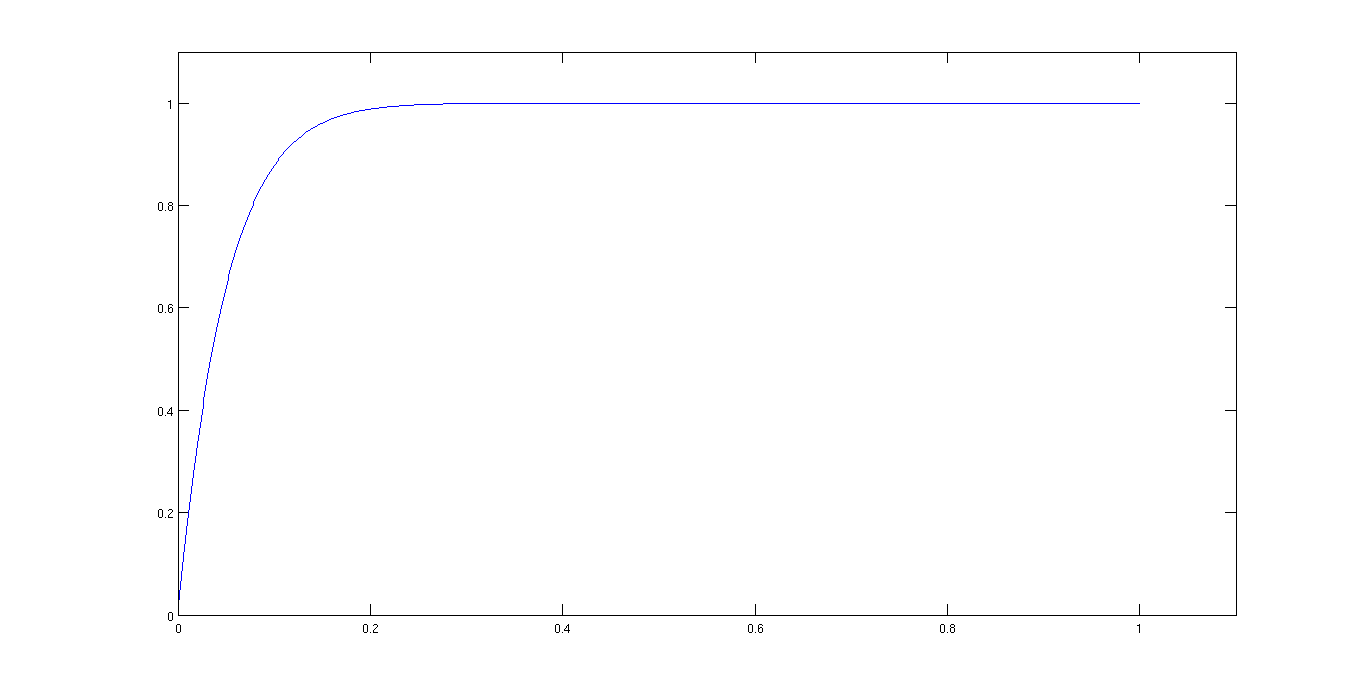
\includegraphics[scale=0.25]{Toy-Birthday}
    \caption{Sample curve of the problem when probability varies, 20 ``independent passwords''}
\label{fig:toy-birthday-attack}
  \end{figure}
\end{itemize}

\subsection{Que 7.9.20}
\label{sec:que-7.9.20}

\begin{itemize}
\item For this question, we have $p$ for the answer since the same
  password is reused.
\item We have $1-{(1-p)}^{n}$.
  \begin{figure}[htbp]
    \centering
    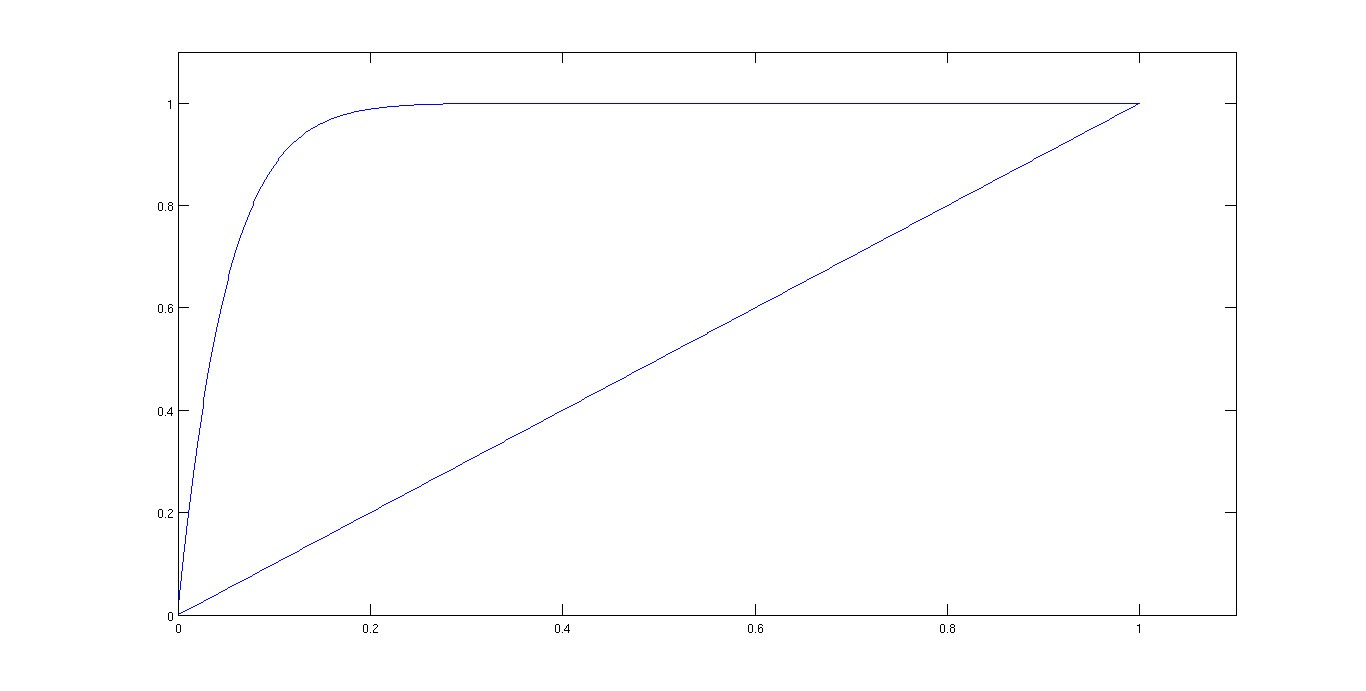
\includegraphics[scale=0.25]{Toy-Birthday-1}
    \caption{Password cracking: use the same password or different ones?}
\label{fig:toy-birthday-attack-1}
  \end{figure}
\item Judging from the figure above, we might come to the
  counter-intuitive conclusion that keeping the same password is
  bringing you more safety, since there is ``just one'' password to be
  matched against dictionary attack. However, for the one-password
  scenario, once this password is cracked, there is no more security
  to talk about.
\end{itemize}

\subsection{Que 7.9.37}
\label{sec:que-7.9.37}

\begin{itemize}
\item For this question we have $d(Alice,Bob)=\frac{1}{16}$, $d(Alice,
  Charlie)=0$ and $d(Bob,Charlie)=$
\end{itemize}










% \BIBLIOGRAPHYSTYLE{AMSALPHA}
% \BIBLIOGRAPHY{HW3-Ref}
\bibliographystyle{amsalpha}
\bibliography{HW3-Ref}


\end{document}
